% Options for packages loaded elsewhere
% Options for packages loaded elsewhere
\PassOptionsToPackage{unicode}{hyperref}
\PassOptionsToPackage{hyphens}{url}
\PassOptionsToPackage{dvipsnames,svgnames,x11names}{xcolor}
%
\documentclass[
  letterpaper,
  DIV=11,
  numbers=noendperiod]{scrartcl}
\usepackage{xcolor}
\usepackage{amsmath,amssymb}
\setcounter{secnumdepth}{-\maxdimen} % remove section numbering
\usepackage{iftex}
\ifPDFTeX
  \usepackage[T1]{fontenc}
  \usepackage[utf8]{inputenc}
  \usepackage{textcomp} % provide euro and other symbols
\else % if luatex or xetex
  \usepackage{unicode-math} % this also loads fontspec
  \defaultfontfeatures{Scale=MatchLowercase}
  \defaultfontfeatures[\rmfamily]{Ligatures=TeX,Scale=1}
\fi
\usepackage{lmodern}
\ifPDFTeX\else
  % xetex/luatex font selection
\fi
% Use upquote if available, for straight quotes in verbatim environments
\IfFileExists{upquote.sty}{\usepackage{upquote}}{}
\IfFileExists{microtype.sty}{% use microtype if available
  \usepackage[]{microtype}
  \UseMicrotypeSet[protrusion]{basicmath} % disable protrusion for tt fonts
}{}
\makeatletter
\@ifundefined{KOMAClassName}{% if non-KOMA class
  \IfFileExists{parskip.sty}{%
    \usepackage{parskip}
  }{% else
    \setlength{\parindent}{0pt}
    \setlength{\parskip}{6pt plus 2pt minus 1pt}}
}{% if KOMA class
  \KOMAoptions{parskip=half}}
\makeatother
% Make \paragraph and \subparagraph free-standing
\makeatletter
\ifx\paragraph\undefined\else
  \let\oldparagraph\paragraph
  \renewcommand{\paragraph}{
    \@ifstar
      \xxxParagraphStar
      \xxxParagraphNoStar
  }
  \newcommand{\xxxParagraphStar}[1]{\oldparagraph*{#1}\mbox{}}
  \newcommand{\xxxParagraphNoStar}[1]{\oldparagraph{#1}\mbox{}}
\fi
\ifx\subparagraph\undefined\else
  \let\oldsubparagraph\subparagraph
  \renewcommand{\subparagraph}{
    \@ifstar
      \xxxSubParagraphStar
      \xxxSubParagraphNoStar
  }
  \newcommand{\xxxSubParagraphStar}[1]{\oldsubparagraph*{#1}\mbox{}}
  \newcommand{\xxxSubParagraphNoStar}[1]{\oldsubparagraph{#1}\mbox{}}
\fi
\makeatother

\usepackage{color}
\usepackage{fancyvrb}
\newcommand{\VerbBar}{|}
\newcommand{\VERB}{\Verb[commandchars=\\\{\}]}
\DefineVerbatimEnvironment{Highlighting}{Verbatim}{commandchars=\\\{\}}
% Add ',fontsize=\small' for more characters per line
\usepackage{framed}
\definecolor{shadecolor}{RGB}{241,243,245}
\newenvironment{Shaded}{\begin{snugshade}}{\end{snugshade}}
\newcommand{\AlertTok}[1]{\textcolor[rgb]{0.68,0.00,0.00}{#1}}
\newcommand{\AnnotationTok}[1]{\textcolor[rgb]{0.37,0.37,0.37}{#1}}
\newcommand{\AttributeTok}[1]{\textcolor[rgb]{0.40,0.45,0.13}{#1}}
\newcommand{\BaseNTok}[1]{\textcolor[rgb]{0.68,0.00,0.00}{#1}}
\newcommand{\BuiltInTok}[1]{\textcolor[rgb]{0.00,0.23,0.31}{#1}}
\newcommand{\CharTok}[1]{\textcolor[rgb]{0.13,0.47,0.30}{#1}}
\newcommand{\CommentTok}[1]{\textcolor[rgb]{0.37,0.37,0.37}{#1}}
\newcommand{\CommentVarTok}[1]{\textcolor[rgb]{0.37,0.37,0.37}{\textit{#1}}}
\newcommand{\ConstantTok}[1]{\textcolor[rgb]{0.56,0.35,0.01}{#1}}
\newcommand{\ControlFlowTok}[1]{\textcolor[rgb]{0.00,0.23,0.31}{\textbf{#1}}}
\newcommand{\DataTypeTok}[1]{\textcolor[rgb]{0.68,0.00,0.00}{#1}}
\newcommand{\DecValTok}[1]{\textcolor[rgb]{0.68,0.00,0.00}{#1}}
\newcommand{\DocumentationTok}[1]{\textcolor[rgb]{0.37,0.37,0.37}{\textit{#1}}}
\newcommand{\ErrorTok}[1]{\textcolor[rgb]{0.68,0.00,0.00}{#1}}
\newcommand{\ExtensionTok}[1]{\textcolor[rgb]{0.00,0.23,0.31}{#1}}
\newcommand{\FloatTok}[1]{\textcolor[rgb]{0.68,0.00,0.00}{#1}}
\newcommand{\FunctionTok}[1]{\textcolor[rgb]{0.28,0.35,0.67}{#1}}
\newcommand{\ImportTok}[1]{\textcolor[rgb]{0.00,0.46,0.62}{#1}}
\newcommand{\InformationTok}[1]{\textcolor[rgb]{0.37,0.37,0.37}{#1}}
\newcommand{\KeywordTok}[1]{\textcolor[rgb]{0.00,0.23,0.31}{\textbf{#1}}}
\newcommand{\NormalTok}[1]{\textcolor[rgb]{0.00,0.23,0.31}{#1}}
\newcommand{\OperatorTok}[1]{\textcolor[rgb]{0.37,0.37,0.37}{#1}}
\newcommand{\OtherTok}[1]{\textcolor[rgb]{0.00,0.23,0.31}{#1}}
\newcommand{\PreprocessorTok}[1]{\textcolor[rgb]{0.68,0.00,0.00}{#1}}
\newcommand{\RegionMarkerTok}[1]{\textcolor[rgb]{0.00,0.23,0.31}{#1}}
\newcommand{\SpecialCharTok}[1]{\textcolor[rgb]{0.37,0.37,0.37}{#1}}
\newcommand{\SpecialStringTok}[1]{\textcolor[rgb]{0.13,0.47,0.30}{#1}}
\newcommand{\StringTok}[1]{\textcolor[rgb]{0.13,0.47,0.30}{#1}}
\newcommand{\VariableTok}[1]{\textcolor[rgb]{0.07,0.07,0.07}{#1}}
\newcommand{\VerbatimStringTok}[1]{\textcolor[rgb]{0.13,0.47,0.30}{#1}}
\newcommand{\WarningTok}[1]{\textcolor[rgb]{0.37,0.37,0.37}{\textit{#1}}}

\usepackage{longtable,booktabs,array}
\usepackage{calc} % for calculating minipage widths
% Correct order of tables after \paragraph or \subparagraph
\usepackage{etoolbox}
\makeatletter
\patchcmd\longtable{\par}{\if@noskipsec\mbox{}\fi\par}{}{}
\makeatother
% Allow footnotes in longtable head/foot
\IfFileExists{footnotehyper.sty}{\usepackage{footnotehyper}}{\usepackage{footnote}}
\makesavenoteenv{longtable}
\usepackage{graphicx}
\makeatletter
\newsavebox\pandoc@box
\newcommand*\pandocbounded[1]{% scales image to fit in text height/width
  \sbox\pandoc@box{#1}%
  \Gscale@div\@tempa{\textheight}{\dimexpr\ht\pandoc@box+\dp\pandoc@box\relax}%
  \Gscale@div\@tempb{\linewidth}{\wd\pandoc@box}%
  \ifdim\@tempb\p@<\@tempa\p@\let\@tempa\@tempb\fi% select the smaller of both
  \ifdim\@tempa\p@<\p@\scalebox{\@tempa}{\usebox\pandoc@box}%
  \else\usebox{\pandoc@box}%
  \fi%
}
% Set default figure placement to htbp
\def\fps@figure{htbp}
\makeatother





\setlength{\emergencystretch}{3em} % prevent overfull lines

\providecommand{\tightlist}{%
  \setlength{\itemsep}{0pt}\setlength{\parskip}{0pt}}



 


\KOMAoption{captions}{tableheading}
\makeatletter
\@ifpackageloaded{caption}{}{\usepackage{caption}}
\AtBeginDocument{%
\ifdefined\contentsname
  \renewcommand*\contentsname{Table of contents}
\else
  \newcommand\contentsname{Table of contents}
\fi
\ifdefined\listfigurename
  \renewcommand*\listfigurename{List of Figures}
\else
  \newcommand\listfigurename{List of Figures}
\fi
\ifdefined\listtablename
  \renewcommand*\listtablename{List of Tables}
\else
  \newcommand\listtablename{List of Tables}
\fi
\ifdefined\figurename
  \renewcommand*\figurename{Figure}
\else
  \newcommand\figurename{Figure}
\fi
\ifdefined\tablename
  \renewcommand*\tablename{Table}
\else
  \newcommand\tablename{Table}
\fi
}
\@ifpackageloaded{float}{}{\usepackage{float}}
\floatstyle{ruled}
\@ifundefined{c@chapter}{\newfloat{codelisting}{h}{lop}}{\newfloat{codelisting}{h}{lop}[chapter]}
\floatname{codelisting}{Listing}
\newcommand*\listoflistings{\listof{codelisting}{List of Listings}}
\makeatother
\makeatletter
\makeatother
\makeatletter
\@ifpackageloaded{caption}{}{\usepackage{caption}}
\@ifpackageloaded{subcaption}{}{\usepackage{subcaption}}
\makeatother
\usepackage{bookmark}
\IfFileExists{xurl.sty}{\usepackage{xurl}}{} % add URL line breaks if available
\urlstyle{same}
\hypersetup{
  pdftitle={Class 12: RNASeq Analysis},
  pdfauthor={Laura Sun (PID:A17923552)},
  colorlinks=true,
  linkcolor={blue},
  filecolor={Maroon},
  citecolor={Blue},
  urlcolor={Blue},
  pdfcreator={LaTeX via pandoc}}


\title{Class 12: RNASeq Analysis}
\author{Laura Sun (PID:A17923552)}
\date{}
\begin{document}
\maketitle

\renewcommand*\contentsname{Table of contents}
{
\hypersetup{linkcolor=}
\setcounter{tocdepth}{3}
\tableofcontents
}

\subsection{Background}\label{background}

Today we will analyze some RNASeq data from himes et al.~on the effects
of a common steroid (dexamethasone) on airway smooth muscle cells (ASM
cells).

Our starting point is the ``counts'' data and ``metadata'' that contain
the count values for each gene in their different experiments (i.e.~cell
lines with or without the drug).

\subsection{Data import}\label{data-import}

Load in console: install.packages(``BiocManager'')
BiocManager::install(``DESeq2'') n

\begin{Shaded}
\begin{Highlighting}[]
\NormalTok{counts }\OtherTok{\textless{}{-}} \FunctionTok{read.csv}\NormalTok{(}\StringTok{"airway\_scaledcounts.csv"}\NormalTok{, }\AttributeTok{row.names=}\DecValTok{1}\NormalTok{)}
\NormalTok{metadata }\OtherTok{\textless{}{-}} \FunctionTok{read.csv}\NormalTok{(}\StringTok{"airway\_metadata.csv"}\NormalTok{)}
\end{Highlighting}
\end{Shaded}

Let's take a look:

\begin{Shaded}
\begin{Highlighting}[]
\FunctionTok{head}\NormalTok{(counts)}
\end{Highlighting}
\end{Shaded}

\begin{verbatim}
                SRR1039508 SRR1039509 SRR1039512 SRR1039513 SRR1039516
ENSG00000000003        723        486        904        445       1170
ENSG00000000005          0          0          0          0          0
ENSG00000000419        467        523        616        371        582
ENSG00000000457        347        258        364        237        318
ENSG00000000460         96         81         73         66        118
ENSG00000000938          0          0          1          0          2
                SRR1039517 SRR1039520 SRR1039521
ENSG00000000003       1097        806        604
ENSG00000000005          0          0          0
ENSG00000000419        781        417        509
ENSG00000000457        447        330        324
ENSG00000000460         94        102         74
ENSG00000000938          0          0          0
\end{verbatim}

\begin{quote}
Q1: How many genes are in this dataset?
\end{quote}

Number of genes:

\begin{Shaded}
\begin{Highlighting}[]
\FunctionTok{nrow}\NormalTok{(counts)}
\end{Highlighting}
\end{Shaded}

\begin{verbatim}
[1] 38694
\end{verbatim}

Experiments:

\begin{Shaded}
\begin{Highlighting}[]
\FunctionTok{nrow}\NormalTok{(metadata)}
\end{Highlighting}
\end{Shaded}

\begin{verbatim}
[1] 8
\end{verbatim}

\begin{quote}
Q2: How many `control' cell lines do we have?
\end{quote}

\begin{Shaded}
\begin{Highlighting}[]
\FunctionTok{sum}\NormalTok{(metadata}\SpecialCharTok{$}\NormalTok{dex}\SpecialCharTok{==}\StringTok{"control"}\NormalTok{)}
\end{Highlighting}
\end{Shaded}

\begin{verbatim}
[1] 4
\end{verbatim}

\subsection{Toy differential gene
expression}\label{toy-differential-gene-expression}

To start our analysis, let's calculate the mean counts for all genes in
the ``control'' experiments.

\begin{enumerate}
\def\labelenumi{\arabic{enumi}.}
\tightlist
\item
  Extract all control columns from the \texttt{counts} object.
\item
  Calculate the mean for all rows (i.e.~genes) of these ``control''
  columns.
\end{enumerate}

3-4. Do the same for ``treated'' group 5. Compare these
\texttt{control.mean} and \texttt{treated.mean} values.

\begin{Shaded}
\begin{Highlighting}[]
\NormalTok{control.inds }\OtherTok{\textless{}{-}}\NormalTok{ metadata}\SpecialCharTok{$}\NormalTok{dex}\SpecialCharTok{==}\StringTok{"control"}
\NormalTok{control.counts }\OtherTok{\textless{}{-}}\NormalTok{ counts[,control.inds]}
\NormalTok{control.means }\OtherTok{\textless{}{-}} \FunctionTok{rowSums}\NormalTok{(control.counts)}\SpecialCharTok{/}\DecValTok{4} \CommentTok{\# Getting the average of each gene\textquotesingle{}s 4 controls. Or use rowMeans(control.counts)}
\end{Highlighting}
\end{Shaded}

\begin{quote}
Q3. How would you make the above code in either approach more robust? Is
there a function that could help here?
\end{quote}

We can use \texttt{rowMeans()} instead of \texttt{rowSums()}/counts to
make it easier.

\begin{quote}
Q4. Follow the same procedure for the treated samples (i.e.~calculate
the mean per gene across drug treated samples and assign to a labeled
vector called treated.mean)
\end{quote}

\begin{Shaded}
\begin{Highlighting}[]
\NormalTok{treated.inds }\OtherTok{\textless{}{-}}\NormalTok{ metadata}\SpecialCharTok{$}\NormalTok{dex}\SpecialCharTok{==}\StringTok{"treated"}
\NormalTok{treated.counts }\OtherTok{\textless{}{-}}\NormalTok{ counts[,treated.inds]}
\NormalTok{treated.means }\OtherTok{\textless{}{-}} \FunctionTok{rowMeans}\NormalTok{(treated.counts)}
\end{Highlighting}
\end{Shaded}

Store these together for ease of bookkeeping as \texttt{meancounts}

\begin{Shaded}
\begin{Highlighting}[]
\NormalTok{meancounts }\OtherTok{\textless{}{-}} \FunctionTok{data.frame}\NormalTok{(control.means, treated.means)}
\FunctionTok{head}\NormalTok{(meancounts)}
\end{Highlighting}
\end{Shaded}

\begin{verbatim}
                control.means treated.means
ENSG00000000003        900.75        658.00
ENSG00000000005          0.00          0.00
ENSG00000000419        520.50        546.00
ENSG00000000457        339.75        316.50
ENSG00000000460         97.25         78.75
ENSG00000000938          0.75          0.00
\end{verbatim}

Make a plot of control vs.~treated mean values for all genes.

\begin{quote}
Q5 (a). Create a scatter plot showing the mean of the treated samples
against the mean of the control samples. Your plot should look something
like the following.
\end{quote}

\begin{Shaded}
\begin{Highlighting}[]
\FunctionTok{plot}\NormalTok{(meancounts[,}\DecValTok{1}\NormalTok{],meancounts[,}\DecValTok{2}\NormalTok{], }\AttributeTok{xlab=}\StringTok{"Control"}\NormalTok{, }\AttributeTok{ylab=}\StringTok{"Treated"}\NormalTok{)}
\end{Highlighting}
\end{Shaded}

\pandocbounded{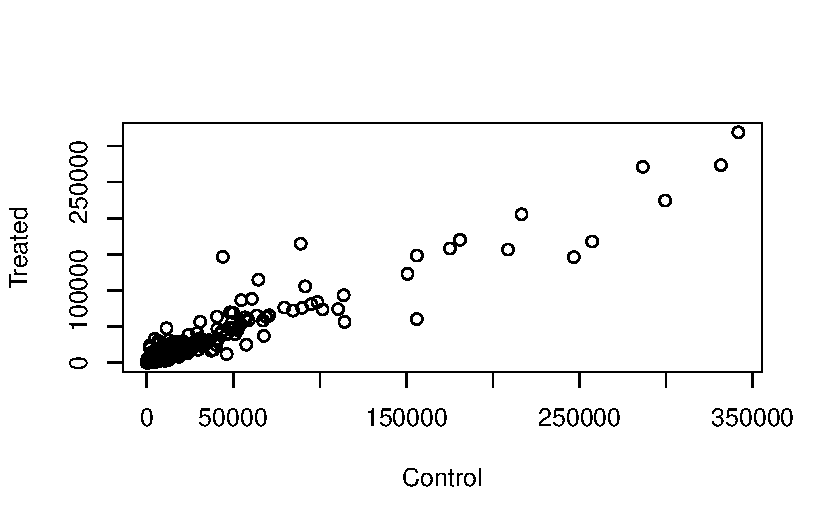
\includegraphics[keepaspectratio]{class12_files/figure-pdf/unnamed-chunk-9-1.pdf}}

\begin{quote}
Q5 (b).You could also use the ggplot2 package to make this figure
producing the plot below. What geom\_?() function would you use for this
plot?
\end{quote}

Use geom\_point() for scatter plot.

\begin{Shaded}
\begin{Highlighting}[]
\FunctionTok{library}\NormalTok{(ggplot2)}
\FunctionTok{ggplot}\NormalTok{(meancounts, }\FunctionTok{aes}\NormalTok{(}\AttributeTok{x=}\NormalTok{control.means, }\AttributeTok{y=}\NormalTok{treated.means)) }\SpecialCharTok{+} \FunctionTok{geom\_point}\NormalTok{() }\SpecialCharTok{+} \FunctionTok{theme\_bw}\NormalTok{()}
\end{Highlighting}
\end{Shaded}

\pandocbounded{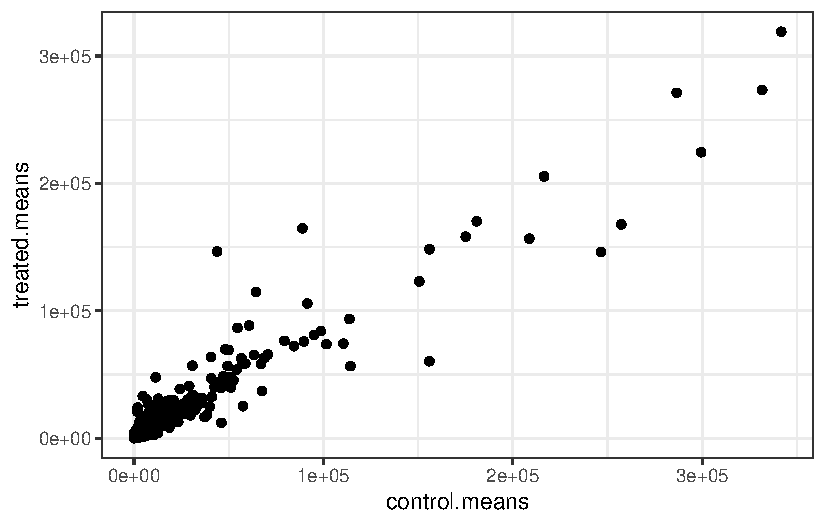
\includegraphics[keepaspectratio]{class12_files/figure-pdf/unnamed-chunk-10-1.pdf}}

\begin{quote}
Q6. Try plotting both axes on a log scale. What is the argument to
plot() that allows you to do this?
\end{quote}

Use scale\_x\_log10() to adjust for skewed data.

\begin{Shaded}
\begin{Highlighting}[]
\FunctionTok{ggplot}\NormalTok{(meancounts, }\FunctionTok{aes}\NormalTok{(}\AttributeTok{x=}\NormalTok{control.means, }\AttributeTok{y=}\NormalTok{treated.means)) }\SpecialCharTok{+} \FunctionTok{geom\_point}\NormalTok{() }\SpecialCharTok{+} \FunctionTok{theme\_bw}\NormalTok{() }\SpecialCharTok{+} \FunctionTok{scale\_x\_log10}\NormalTok{() }\SpecialCharTok{+} \FunctionTok{scale\_y\_log10}\NormalTok{()}
\end{Highlighting}
\end{Shaded}

\begin{verbatim}
Warning in scale_x_log10(): log-10 transformation introduced infinite values.
\end{verbatim}

\begin{verbatim}
Warning in scale_y_log10(): log-10 transformation introduced infinite values.
\end{verbatim}

\pandocbounded{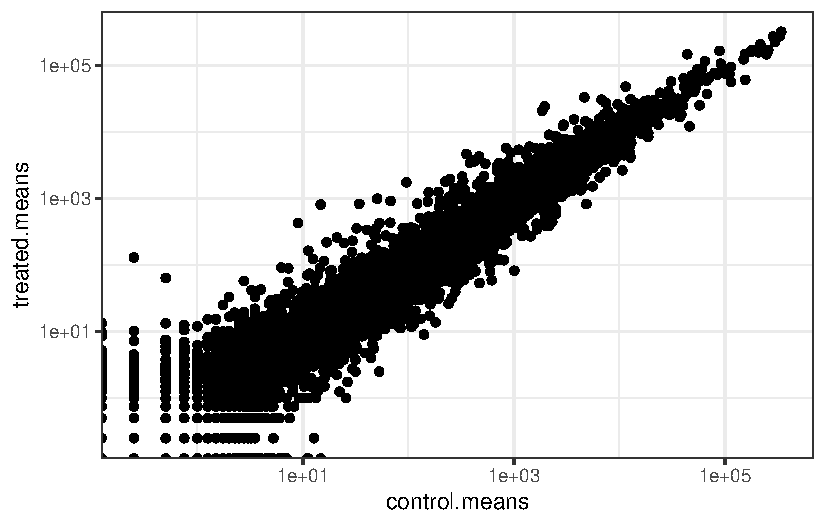
\includegraphics[keepaspectratio]{class12_files/figure-pdf/unnamed-chunk-11-1.pdf}}

\begin{Shaded}
\begin{Highlighting}[]
\CommentTok{\# or plot(meancounts, log="xy")}
\end{Highlighting}
\end{Shaded}

We often talk about metrics like ``log2 fold-change''

\begin{Shaded}
\begin{Highlighting}[]
\CommentTok{\# control/treated}
\FunctionTok{log2}\NormalTok{(}\DecValTok{10}\SpecialCharTok{/}\DecValTok{10}\NormalTok{) }\CommentTok{\# gives 0, so 0 change.}
\end{Highlighting}
\end{Shaded}

\begin{verbatim}
[1] 0
\end{verbatim}

\begin{Shaded}
\begin{Highlighting}[]
\FunctionTok{log2}\NormalTok{(}\DecValTok{40}\SpecialCharTok{/}\DecValTok{10}\NormalTok{)}
\end{Highlighting}
\end{Shaded}

\begin{verbatim}
[1] 2
\end{verbatim}

\begin{Shaded}
\begin{Highlighting}[]
\FunctionTok{log2}\NormalTok{(}\DecValTok{10}\SpecialCharTok{/}\DecValTok{40}\NormalTok{)}
\end{Highlighting}
\end{Shaded}

\begin{verbatim}
[1] -2
\end{verbatim}

Let's calculate the log2 fold change for our treated oven control mean
counts.

\begin{Shaded}
\begin{Highlighting}[]
\NormalTok{meancounts}\SpecialCharTok{$}\NormalTok{log2fc }\OtherTok{\textless{}{-}} \FunctionTok{log2}\NormalTok{(meancounts}\SpecialCharTok{$}\NormalTok{treated.means}\SpecialCharTok{/}\NormalTok{ meancounts}\SpecialCharTok{$}\NormalTok{control.means)}
\CommentTok{\# add a column.}

\FunctionTok{head}\NormalTok{(meancounts)}
\end{Highlighting}
\end{Shaded}

\begin{verbatim}
                control.means treated.means      log2fc
ENSG00000000003        900.75        658.00 -0.45303916
ENSG00000000005          0.00          0.00         NaN
ENSG00000000419        520.50        546.00  0.06900279
ENSG00000000457        339.75        316.50 -0.10226805
ENSG00000000460         97.25         78.75 -0.30441833
ENSG00000000938          0.75          0.00        -Inf
\end{verbatim}

\begin{Shaded}
\begin{Highlighting}[]
\NormalTok{zero.vals }\OtherTok{\textless{}{-}} \FunctionTok{which}\NormalTok{(meancounts[,}\DecValTok{1}\SpecialCharTok{:}\DecValTok{2}\NormalTok{]}\SpecialCharTok{==}\DecValTok{0}\NormalTok{, }\AttributeTok{arr.ind=}\ConstantTok{TRUE}\NormalTok{)}
\NormalTok{to.rm }\OtherTok{\textless{}{-}} \FunctionTok{unique}\NormalTok{(zero.vals[,}\DecValTok{1}\NormalTok{])}
\NormalTok{mycounts }\OtherTok{\textless{}{-}}\NormalTok{ meancounts[}\SpecialCharTok{{-}}\NormalTok{to.rm,]}
\FunctionTok{head}\NormalTok{(mycounts)}
\end{Highlighting}
\end{Shaded}

\begin{verbatim}
                control.means treated.means      log2fc
ENSG00000000003        900.75        658.00 -0.45303916
ENSG00000000419        520.50        546.00  0.06900279
ENSG00000000457        339.75        316.50 -0.10226805
ENSG00000000460         97.25         78.75 -0.30441833
ENSG00000000971       5219.00       6687.50  0.35769358
ENSG00000001036       2327.00       1785.75 -0.38194109
\end{verbatim}

\begin{quote}
Q7: What is the purpose of the arr.ind argument in the which() function
call above? Why would we then take the first column of the output and
need to call the unique() function?
\end{quote}

The arr.ind=TRUE with which() return the indices of TRUE values, showing
the location of zeros. We ignore genes with zero counts. unique() helps
to not count a row twice if it has zeros.

A common ``rule of thumb'' is a log2 full change cutoff of +2 and -2 to
call genes ``Up regulated'' or ``Down regulated''.

\begin{quote}
Q8: Number of ``up regulated'' genes:
\end{quote}

\begin{Shaded}
\begin{Highlighting}[]
\FunctionTok{sum}\NormalTok{(meancounts}\SpecialCharTok{$}\NormalTok{log2fc }\SpecialCharTok{\textgreater{}} \SpecialCharTok{+}\DecValTok{2}\NormalTok{, }\AttributeTok{na.rm=}\NormalTok{T)}
\end{Highlighting}
\end{Shaded}

\begin{verbatim}
[1] 1846
\end{verbatim}

\begin{Shaded}
\begin{Highlighting}[]
\CommentTok{\#na.rm=T means don\textquotesingle{}t count the NAs.}
\end{Highlighting}
\end{Shaded}

\begin{quote}
Q9: Number of down regulated genes:
\end{quote}

\begin{Shaded}
\begin{Highlighting}[]
\FunctionTok{sum}\NormalTok{(meancounts}\SpecialCharTok{$}\NormalTok{log2fc }\SpecialCharTok{\textless{}} \SpecialCharTok{{-}}\DecValTok{2}\NormalTok{, }\AttributeTok{na.rm=}\NormalTok{T)}
\end{Highlighting}
\end{Shaded}

\begin{verbatim}
[1] 2212
\end{verbatim}

\begin{quote}
Q10: We are missing statistical significance of the data. We don't know
if the difference between control and treated are caused by random
errors, skewed data, or there's a real significant difference. We can
use something like two sample t-test to check for statistical
significance.
\end{quote}

\subsection{DESeq2 analysis}\label{deseq2-analysis}

\begin{Shaded}
\begin{Highlighting}[]
\FunctionTok{library}\NormalTok{(DESeq2)}
\end{Highlighting}
\end{Shaded}

For DESeq analysis we need three things:

\begin{enumerate}
\def\labelenumi{\arabic{enumi}.}
\tightlist
\item
  count values (\texttt{countData})
\item
  metadata telling us about the columns in \texttt{countData}
  (\texttt{colData})
\item
  design of the experiment (i.e.~what do you want to compare)
\end{enumerate}

Our first function from DESeq2 will setup the input required for
analysis by storing all these 3 things together.

\begin{Shaded}
\begin{Highlighting}[]
\NormalTok{dds }\OtherTok{\textless{}{-}} \FunctionTok{DESeqDataSetFromMatrix}\NormalTok{(}\AttributeTok{countData =}\NormalTok{ counts, }\AttributeTok{colData =}\NormalTok{ metadata, }\AttributeTok{design =} \SpecialCharTok{\textasciitilde{}}\NormalTok{dex)}
\end{Highlighting}
\end{Shaded}

\begin{verbatim}
converting counts to integer mode
\end{verbatim}

\begin{verbatim}
Warning in DESeqDataSet(se, design = design, ignoreRank): some variables in
design formula are characters, converting to factors
\end{verbatim}

The main function in DESeq2 that runs the analysis is called
\texttt{DESeq()}

\begin{Shaded}
\begin{Highlighting}[]
\NormalTok{dds }\OtherTok{\textless{}{-}} \FunctionTok{DESeq}\NormalTok{(dds)}
\end{Highlighting}
\end{Shaded}

\begin{verbatim}
estimating size factors
\end{verbatim}

\begin{verbatim}
estimating dispersions
\end{verbatim}

\begin{verbatim}
gene-wise dispersion estimates
\end{verbatim}

\begin{verbatim}
mean-dispersion relationship
\end{verbatim}

\begin{verbatim}
final dispersion estimates
\end{verbatim}

\begin{verbatim}
fitting model and testing
\end{verbatim}

\begin{Shaded}
\begin{Highlighting}[]
\NormalTok{res }\OtherTok{\textless{}{-}} \FunctionTok{results}\NormalTok{(dds)}
\FunctionTok{head}\NormalTok{(res)}
\end{Highlighting}
\end{Shaded}

\begin{verbatim}
log2 fold change (MLE): dex treated vs control 
Wald test p-value: dex treated vs control 
DataFrame with 6 rows and 6 columns
                  baseMean log2FoldChange     lfcSE      stat    pvalue
                 <numeric>      <numeric> <numeric> <numeric> <numeric>
ENSG00000000003 747.194195      -0.350703  0.168242 -2.084514 0.0371134
ENSG00000000005   0.000000             NA        NA        NA        NA
ENSG00000000419 520.134160       0.206107  0.101042  2.039828 0.0413675
ENSG00000000457 322.664844       0.024527  0.145134  0.168996 0.8658000
ENSG00000000460  87.682625      -0.147143  0.256995 -0.572550 0.5669497
ENSG00000000938   0.319167      -1.732289  3.493601 -0.495846 0.6200029
                     padj
                <numeric>
ENSG00000000003  0.163017
ENSG00000000005        NA
ENSG00000000419  0.175937
ENSG00000000457  0.961682
ENSG00000000460  0.815805
ENSG00000000938        NA
\end{verbatim}

\begin{Shaded}
\begin{Highlighting}[]
\DecValTok{36000}\SpecialCharTok{*}\FloatTok{0.05}
\end{Highlighting}
\end{Shaded}

\begin{verbatim}
[1] 1800
\end{verbatim}

\subsection{Volcano Plot}\label{volcano-plot}

This is a common summary result figure from these types of experiments
and plot the log2 fold-change vs.~the adjusted p-value.

\begin{Shaded}
\begin{Highlighting}[]
\FunctionTok{plot}\NormalTok{(res}\SpecialCharTok{$}\NormalTok{log2FoldChange, }\SpecialCharTok{{-}}\FunctionTok{log}\NormalTok{(res}\SpecialCharTok{$}\NormalTok{padj))}
\CommentTok{\# use {-}log to change the axis}

\FunctionTok{abline}\NormalTok{(}\AttributeTok{v=}\FunctionTok{c}\NormalTok{(}\SpecialCharTok{{-}}\DecValTok{2}\NormalTok{,}\DecValTok{2}\NormalTok{), }\AttributeTok{col=}\StringTok{"red"}\NormalTok{)}
\FunctionTok{abline}\NormalTok{(}\AttributeTok{h=}\SpecialCharTok{{-}}\FunctionTok{log}\NormalTok{(}\FloatTok{0.04}\NormalTok{), }\AttributeTok{col=}\StringTok{"red"}\NormalTok{)}
\end{Highlighting}
\end{Shaded}

\pandocbounded{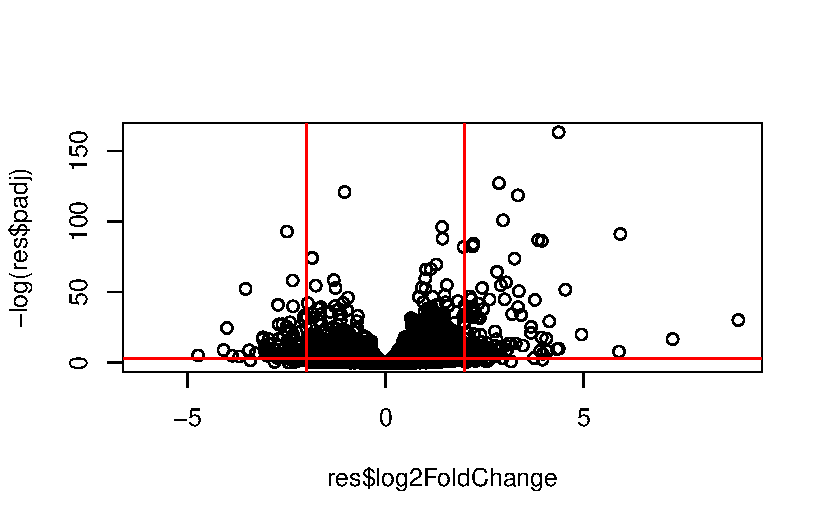
\includegraphics[keepaspectratio]{class12_files/figure-pdf/unnamed-chunk-23-1.pdf}}

\subsection{Save our result}\label{save-our-result}

\begin{Shaded}
\begin{Highlighting}[]
\FunctionTok{write.csv}\NormalTok{(res, }\AttributeTok{file=}\StringTok{"my\_results.csv"}\NormalTok{)}
\end{Highlighting}
\end{Shaded}

\subsection{Add gene annotation}\label{add-gene-annotation}

To help make sense of our results and communicate them to other folk, we
need to add more annotations to our main \texttt{res} object.

We will use two bioconductor packages to first map IDs to different
formats including classic gene ``symbol'' gene name.

Install these with the following commands:
\texttt{BiocManager::install("AnnotationDbi")}
\texttt{BiocManager::install("org.Hs.eg.db")}

\begin{Shaded}
\begin{Highlighting}[]
\FunctionTok{library}\NormalTok{(}\StringTok{"AnnotationDbi"}\NormalTok{)}
\FunctionTok{library}\NormalTok{(}\StringTok{"org.Hs.eg.db"}\NormalTok{)}
\end{Highlighting}
\end{Shaded}

\begin{verbatim}
\end{verbatim}

\begin{Shaded}
\begin{Highlighting}[]
\CommentTok{\#mygenes$control \textless{}{-} maplds(org.Hs.eg.db, column="SYMBOL", \#keys=row.names(mygenes), keytype"ENSEMBL")}
\end{Highlighting}
\end{Shaded}

Let's see what's in \texttt{org.Hs.eg.db} with the \texttt{columns()}
function''

\begin{Shaded}
\begin{Highlighting}[]
\FunctionTok{columns}\NormalTok{(org.Hs.eg.db)}
\end{Highlighting}
\end{Shaded}

\begin{verbatim}
 [1] "ACCNUM"       "ALIAS"        "ENSEMBL"      "ENSEMBLPROT"  "ENSEMBLTRANS"
 [6] "ENTREZID"     "ENZYME"       "EVIDENCE"     "EVIDENCEALL"  "GENENAME"    
[11] "GENETYPE"     "GO"           "GOALL"        "IPI"          "MAP"         
[16] "OMIM"         "ONTOLOGY"     "ONTOLOGYALL"  "PATH"         "PFAM"        
[21] "PMID"         "PROSITE"      "REFSEQ"       "SYMBOL"       "UCSCKG"      
[26] "UNIPROT"     
\end{verbatim}

We can translate or ``map'' IDs between any of these 26 databases using
the \texttt{mapIDs()} function.

\begin{Shaded}
\begin{Highlighting}[]
\FunctionTok{head}\NormalTok{(}\FunctionTok{row.names}\NormalTok{(res))}
\end{Highlighting}
\end{Shaded}

\begin{verbatim}
[1] "ENSG00000000003" "ENSG00000000005" "ENSG00000000419" "ENSG00000000457"
[5] "ENSG00000000460" "ENSG00000000938"
\end{verbatim}

\begin{Shaded}
\begin{Highlighting}[]
\NormalTok{res}\SpecialCharTok{$}\NormalTok{symbol }\OtherTok{\textless{}{-}} \FunctionTok{mapIds}\NormalTok{(}\AttributeTok{keys=}\FunctionTok{row.names}\NormalTok{(res), }\CommentTok{\# our current IDs}
       \AttributeTok{keytype=}\StringTok{"ENSEMBL"}\NormalTok{, }\CommentTok{\# the format of our IDs}
       \AttributeTok{x=}\NormalTok{org.Hs.eg.db, }\CommentTok{\# where to get the mappings from}
       \AttributeTok{column=}\StringTok{"SYMBOL"}\NormalTok{) }\CommentTok{\# the format/DB to map to}
\end{Highlighting}
\end{Shaded}

\begin{verbatim}
'select()' returned 1:many mapping between keys and columns
\end{verbatim}

\begin{Shaded}
\begin{Highlighting}[]
\FunctionTok{head}\NormalTok{(res)}
\end{Highlighting}
\end{Shaded}

\begin{verbatim}
log2 fold change (MLE): dex treated vs control 
Wald test p-value: dex treated vs control 
DataFrame with 6 rows and 7 columns
                  baseMean log2FoldChange     lfcSE      stat    pvalue
                 <numeric>      <numeric> <numeric> <numeric> <numeric>
ENSG00000000003 747.194195      -0.350703  0.168242 -2.084514 0.0371134
ENSG00000000005   0.000000             NA        NA        NA        NA
ENSG00000000419 520.134160       0.206107  0.101042  2.039828 0.0413675
ENSG00000000457 322.664844       0.024527  0.145134  0.168996 0.8658000
ENSG00000000460  87.682625      -0.147143  0.256995 -0.572550 0.5669497
ENSG00000000938   0.319167      -1.732289  3.493601 -0.495846 0.6200029
                     padj      symbol
                <numeric> <character>
ENSG00000000003  0.163017      TSPAN6
ENSG00000000005        NA        TNMD
ENSG00000000419  0.175937        DPM1
ENSG00000000457  0.961682       SCYL3
ENSG00000000460  0.815805       FIRRM
ENSG00000000938        NA         FGR
\end{verbatim}

Add the mappings for ``GENENAME'' and ``ENTREZID'' and store as
\texttt{res\$genename} and \texttt{res\$entrez}

\begin{Shaded}
\begin{Highlighting}[]
\NormalTok{res}\SpecialCharTok{$}\NormalTok{genename }\OtherTok{\textless{}{-}} \FunctionTok{mapIds}\NormalTok{(}\AttributeTok{keys=}\FunctionTok{row.names}\NormalTok{(res), }\CommentTok{\# our current IDs}
       \AttributeTok{keytype=}\StringTok{"ENSEMBL"}\NormalTok{, }\CommentTok{\# the format of our IDs}
       \AttributeTok{x=}\NormalTok{org.Hs.eg.db, }\CommentTok{\# where to get the mappings from}
       \AttributeTok{column=}\StringTok{"GENENAME"}\NormalTok{) }\CommentTok{\# the format/DB to map to}
\end{Highlighting}
\end{Shaded}

\begin{verbatim}
'select()' returned 1:many mapping between keys and columns
\end{verbatim}

\begin{Shaded}
\begin{Highlighting}[]
\NormalTok{res}\SpecialCharTok{$}\NormalTok{entrez }\OtherTok{\textless{}{-}} \FunctionTok{mapIds}\NormalTok{(}\AttributeTok{keys=}\FunctionTok{row.names}\NormalTok{(res), }\CommentTok{\# our current IDs}
       \AttributeTok{keytype=}\StringTok{"ENSEMBL"}\NormalTok{, }\CommentTok{\# the format of our IDs}
       \AttributeTok{x=}\NormalTok{org.Hs.eg.db, }\CommentTok{\# where to get the mappings from}
       \AttributeTok{column=}\StringTok{"ENTREZID"}\NormalTok{) }\CommentTok{\# the format/DB to map to}
\end{Highlighting}
\end{Shaded}

\begin{verbatim}
'select()' returned 1:many mapping between keys and columns
\end{verbatim}

\subsection{Pathway Analysis}\label{pathway-analysis}

There are lots of bioconductor packages to do this type of analysis. For
now let's try one called \textbf{gage}. Again, we need t o install this
if we don't have it already.

BiocManager::install(``gage'') BiocManager::install(``gageData'')
BiocManager::install(``pathview'')

\begin{Shaded}
\begin{Highlighting}[]
\FunctionTok{library}\NormalTok{(gage)}
\FunctionTok{library}\NormalTok{(gageData)}
\FunctionTok{library}\NormalTok{(pathview)}
\end{Highlighting}
\end{Shaded}

To use \textbf{gage} I need two things

\begin{itemize}
\tightlist
\item
  a named vector of fold-change DEGs (our geneset of interest)
\item
  a set of pathways of genesets to use for
\end{itemize}

\begin{Shaded}
\begin{Highlighting}[]
\NormalTok{x }\OtherTok{\textless{}{-}} \FunctionTok{c}\NormalTok{(}\StringTok{"barry"}\OtherTok{=}\DecValTok{5}\NormalTok{, }\StringTok{"lisa"}\OtherTok{=}\DecValTok{10}\NormalTok{)}
\NormalTok{x}
\end{Highlighting}
\end{Shaded}

\begin{verbatim}
barry  lisa 
    5    10 
\end{verbatim}

\begin{Shaded}
\begin{Highlighting}[]
\FunctionTok{names}\NormalTok{(x) }\OtherTok{\textless{}{-}} \FunctionTok{c}\NormalTok{(}\StringTok{"low"}\NormalTok{, }\StringTok{"high"}\NormalTok{)}
\NormalTok{x}
\end{Highlighting}
\end{Shaded}

\begin{verbatim}
 low high 
   5   10 
\end{verbatim}

\begin{Shaded}
\begin{Highlighting}[]
\NormalTok{foldchanges }\OtherTok{\textless{}{-}}\NormalTok{ res}\SpecialCharTok{$}\NormalTok{log2FoldChange}
\FunctionTok{names}\NormalTok{(foldchanges) }\OtherTok{\textless{}{-}}\NormalTok{ res}\SpecialCharTok{$}\NormalTok{entrez}
\FunctionTok{head}\NormalTok{(foldchanges)}
\end{Highlighting}
\end{Shaded}

\begin{verbatim}
       7105       64102        8813       57147       55732        2268 
-0.35070296          NA  0.20610728  0.02452701 -0.14714263 -1.73228897 
\end{verbatim}

\begin{Shaded}
\begin{Highlighting}[]
\FunctionTok{data}\NormalTok{(kegg.sets.hs)}
\NormalTok{keggres}\OtherTok{=}\FunctionTok{gage}\NormalTok{(foldchanges,}\AttributeTok{gsets=}\NormalTok{kegg.sets.hs)}
\end{Highlighting}
\end{Shaded}

In our results object we have:

\begin{Shaded}
\begin{Highlighting}[]
\FunctionTok{attributes}\NormalTok{(keggres)}
\end{Highlighting}
\end{Shaded}

\begin{verbatim}
$names
[1] "greater" "less"    "stats"  
\end{verbatim}

\begin{Shaded}
\begin{Highlighting}[]
\FunctionTok{head}\NormalTok{(keggres}\SpecialCharTok{$}\NormalTok{less,}\DecValTok{5}\NormalTok{)}
\end{Highlighting}
\end{Shaded}

\begin{verbatim}
                                                         p.geomean stat.mean
hsa05332 Graft-versus-host disease                    0.0004250607 -3.473335
hsa04940 Type I diabetes mellitus                     0.0017820379 -3.002350
hsa05310 Asthma                                       0.0020046180 -3.009045
hsa04672 Intestinal immune network for IgA production 0.0060434609 -2.560546
hsa05330 Allograft rejection                          0.0073679547 -2.501416
                                                             p.val      q.val
hsa05332 Graft-versus-host disease                    0.0004250607 0.09053792
hsa04940 Type I diabetes mellitus                     0.0017820379 0.14232788
hsa05310 Asthma                                       0.0020046180 0.14232788
hsa04672 Intestinal immune network for IgA production 0.0060434609 0.31387487
hsa05330 Allograft rejection                          0.0073679547 0.31387487
                                                      set.size         exp1
hsa05332 Graft-versus-host disease                          40 0.0004250607
hsa04940 Type I diabetes mellitus                           42 0.0017820379
hsa05310 Asthma                                             29 0.0020046180
hsa04672 Intestinal immune network for IgA production       47 0.0060434609
hsa05330 Allograft rejection                                36 0.0073679547
\end{verbatim}

Let's look at one of these pathways (hsa05310 Asthma) with our gene
colored up so we can see the overlap

\begin{Shaded}
\begin{Highlighting}[]
\FunctionTok{pathview}\NormalTok{(}\AttributeTok{pathway.id=}\StringTok{"hsa05310"}\NormalTok{, }\AttributeTok{gene.data=}\NormalTok{foldchanges)}
\end{Highlighting}
\end{Shaded}

\begin{verbatim}
'select()' returned 1:1 mapping between keys and columns
\end{verbatim}

\begin{verbatim}
Info: Working in directory /Users/laurasun/Desktop/3rd Year/BIMM143/bimm143_github/wk6class12
\end{verbatim}

\begin{verbatim}
Info: Writing image file hsa05310.pathview.png
\end{verbatim}

Add this pathway figure to our lab report:

\pandocbounded{\includegraphics[keepaspectratio]{.pdf}}

\subsection{Save our main results}\label{save-our-main-results}

\begin{Shaded}
\begin{Highlighting}[]
\FunctionTok{write.csv}\NormalTok{(res, }\AttributeTok{file=}\StringTok{"myresults\_annotated.csv"}\NormalTok{)}
\end{Highlighting}
\end{Shaded}





\end{document}
